% !TEX program = xelatex
% DuplexPilot V3. Publication-style revision of the supplied V2 manuscript.
% Experimental observations are unchanged. Evidence provenance is in Appendix A
% and in the separate author-facing audit directory.
\documentclass{article}
\usepackage{iclr2027_conference,times}
\usepackage[UTF8,fontset=fandol]{ctex}
\usepackage{amsmath,amssymb,graphicx,booktabs,array,multirow}
\usepackage{algorithm,algpseudocode}
\floatname{algorithm}{算法}
\algrenewcommand{\algorithmicrequire}{\textbf{输入:}}
\algrenewcommand{\algorithmicensure}{\textbf{保证:}}
\algrenewcommand{\algorithmicif}{\textbf{若}}
\algrenewcommand{\algorithmicthen}{\textbf{则}}
\algrenewcommand{\algorithmicend}{\textbf{结束}}
\algrenewcommand{\algorithmicwhile}{\textbf{当}}
\algrenewcommand{\algorithmicdo}{\textbf{执行}}
\algrenewcommand{\algorithmicelse}{\textbf{否则}}
\algrenewcommand{\algorithmicreturn}{\textbf{返回}}
\usepackage{xcolor,hyperref,url,xurl}
\usepackage{placeins,float}
\hypersetup{hidelinks,pdftitle={DuplexPilot：面向全双工语音计划内冷恢复的请求归属状态虚拟化},pdfsubject={原生全双工语音会话状态与冷恢复}}
\urlstyle{same}
\newcommand{\sys}{\textsc{DuplexPilot}}
\newcommand{\na}{\textemdash}
\newcommand{\state}[1]{\mathsf{#1}}
\title{DuplexPilot：面向全双工语音计划内冷恢复的请求归属状态虚拟化}
% Keep the review format. Do not enable \iclrfinalcopy for initial submission.
\begin{document}
\maketitle
\begin{abstract}
全双工语音服务的执行状态相互关联，并分布于语言生成、
token缓冲与声学合成等多个阶段。
因此，在挂起期间回收会话私有资源时，
仅恢复语言模型的键值缓存并不足够：
待完成的计算还必须与新接收的输入及已经交付的音频保持一致。
本文提出\textsc{DuplexPilot}，一种基于请求归属状态虚拟化、
支持一致冷恢复的语音服务运行时。
DuplexPilot将逻辑会话状态与物理执行资源分离，
在一致切面上捕获模型、桥接与声学状态。
其恢复协议保留输入与交付记录，建立独立的主机内存检查点，
并在恢复后的状态与执行绑定通过验证后，
才允许继续计算和提交输出。
共享模型权重保持常驻，无需重新训练或改变采样语义。
有界打包检查点传输与完整性校验模块进一步降低恢复开销。
受控实验表明，在所评估配置下，
系统能够保持token与波形续算结果的一致性。
相比逐轮完整历史重建，DuplexPilot将从Worklet恢复到首个新计算
PCM帧渲染的区间缩短了12.5秒，该数值为配对减少量的中位数。
在另一组匹配的传输微基准中，优化的传输与校验模块相较同步实现，
将检查点传输开始到接收端就绪的区间降低了16\%，该数值为逐对相对
降幅的中位数；该实验没有测量PCM渲染或端到端恢复时延。
上述结果为可恢复全双工语音服务提供了显式执行状态基础，
并刻画了跨阶段会话恢复中的资源--时延权衡。
\end{abstract}

\section{引言}
\label{sec:introduction}

全双工语音交互支持同时听说，包括重叠语音、打断和附和
\citep{dgslm2023,syncllm2024}。Moshi与Lychee-FD等模型协调语言和声学
多路流 \citep{moshi2024,lychee2026}，因此服务运行时必须保持模型进度、
声学消费和音频交付的一致性。

本文研究\emph{计划内冷恢复}：在明确挂起时释放会话私有GPU状态，
并在权重保持加载时从主机状态继续执行。热驻留避免重建，完整重建
重新构造被释放状态，部分卸载则保留选定阶段；与普通对话停顿不同，
该操作会停止执行并在稍后恢复。本文统一使用以下术语：\emph{计划内冷恢复}
（planned cold resumption）指明确暂停、释放请求私有状态并随后恢复；
\emph{Save}指从暂停接受到独立检查点就绪，\emph{Ready}指从恢复接受到
执行就绪，\emph{Gap}指缓存PCM耗尽到首个新计算PCM之间的区间。\emph{first-new-PCM}
指真正新计算PCM的第一帧被AudioContext渲染；缓存或重放音频不计入。
\emph{外部账本}（external ledger）记录计算回退不改变的当前事实，包括已接受
输入、取消和交付／渲染记录。\emph{续算保真性}（continuation fidelity）只表示
token与PCM的数值连续性，不表示语义等价或听感等价。本文用\emph{检查点传输}
表示检查点字节搬运，用\emph{request ID}表示逻辑身份，并统一写作\emph{Flow / HiFT}。PagedAttention、SGLang、CachedAttention、
InferCept和Llumnix提供KV复用、拦截、卸载或请求迁移
\citep{vllm2023,sglang2024,cachedattention2024,infercept2024,llumnix2024}；
LiveServe、vLLM-Omni和Execution-State Capsules分别提供语音感知调度、
重连或计算图边界恢复 \citep{liveserve2026,omnidoc,capsules2026}。
这些机制尚未共同定义覆盖模型状态、桥接内容、声学连续状态及外部
输入和交付事实的一致切面。

因此本文提出三个问题：联合状态能否保持新生成token和波形后缀；
释放私有资源的时延与内存代价是什么；有界传输能否减少等待、又会带来
多少暂存开销？本文只研究常驻服务内逻辑请求的计划内挂起，不覆盖任意
进程崩溃、客户端断线容灾、语义质量和不受限并发计划内冷恢复。

核心困难是\emph{跨阶段一致性}：token可能仍在桥接中，而合成和播放
尚未完成；物理执行行、采样选择、KV块和声学上下文可以变化，但逻辑身份
保持不变，已接受输入和已交付音频不能回退。应用一致快照和恢复原则
\citep{chandy1985,elnozahy2002}需要显式的归属、进度和提交规则；
图~\ref{fig:motivation}概括这些依赖及声学执行粒度。

\begin{figure}[t]
    \centering
    \includegraphics[width=\linewidth]{fig1.pdf}
    \caption{
        \textbf{显式状态虚拟化的研究动机。}
        (a) 将逻辑状态绑定到临时执行位置，可能在暂停与复用时导致身份失效、
        桥接内容遗漏或过期输出事件。(b) 在所分析的执行栈中，Flow与HiFT耗时
        分别约为$190$\,ms和$27$\,ms；受支持的$22$--$24.5$\,ms Euler步边界
        提供了更细的捕获与恢复粒度。这些是阶段级观察而非端到端加速，步级分块为示意。
    }
    \label{fig:motivation}
\end{figure}

本文提出\textsc{DuplexPilot}，一种请求归属状态虚拟化运行时：在一致切面
捕获模型状态、桥接待处理内容、声学连续状态和阶段进度，并将输入接收与
交付记录置于计算回退之外。系统在释放私有资源前建立独立主机检查点，
恢复时重建合法绑定并在执行或输出提交前联合验证；有界打包与完整性校验
降低搬运开销而不改变恢复合同或采样语义。

同模型受控实验比较热驻留、部分卸载、联合卸载和逐轮重建。在所测试条件下，
DuplexPilot保持token和波形续算；相对重建参考，从Worklet恢复到首个新计算
PCM帧渲染的区间配对减少中位数约12.5秒；独立的传输微基准中，检查点传输到
接收端就绪区间的配对相对降幅中位数为16\%，该实验不测量渲染。
本文贡献包括：
\begin{itemize}
    \item 跨物理资源变化关联模型执行、桥接内容和声学连续状态的请求归属表示。
    \item 在保留外部输入与交付事实的同时，协调捕获、资源交还、恢复和验证后提交的联合冷恢复协议。
    \item 在固定恢复合同下对续算保真性、驻留权衡和传输效率的评价。
\end{itemize}

\section{相关工作}
\label{sec:related_work}

\noindent\textbf{全双工语音模型与评价。}
Duplex Conversation协调对话状态检测、附和与插话处理
\citep{duplexconversation2022}；后续双工模型采用时间切片实现听说并行
\citep{duplexmodel2024}。dGSLM和SyncLLM分别研究
双通道语音建模与真实时间同步\citep{dgslm2023,syncllm2024}。
Moshi结合语音生成与文本规划\citep{moshi2024}；SpeechGPT和PSLM
分别探索跨模态及文本--语音并行生成\citep{speechgpt2023,pslm2024}；
LLaMA-Omni、LLaMA-Omni 2和OmniFlatten进一步面向低时延或端到端
语音交互\citep{llamaomni2025,llamaomni2_2025,omniflatten2025}。
Freeze-Omni将训练后的语音组件连接到冻结的语言骨干
\citep{freezeomni2025}，Lychee-FD则分离声学与语义建模
\citep{lychee2026}。
FD-Bench评价回应、打断行为及其时序\citep{fdbench2025}；
Full-Duplex-Bench家族包括原始v1、关注重叠处理的v1.5版本
\citep{fdbv1_2025,fdbv15_2025}，以及进一步考察多轮指令遵循与任务能力的
Full-Duplex-Bench-v2框架\citep{fdbv2_2026}。近期综述系统梳理了语音语言模型的架构、训练和评价
空间\citep{arora2025slm}。
这些研究与DuplexPilot的执行状态管理形成互补；
后者无需重新训练底层模型。
对话质量与续算保真性仍然属于不同的评价维度。
本文研究执行状态恢复，不改变模型本身或对话能力。

\noindent\textbf{状态化与语音感知服务。}
Orca、vLLM和SGLang分别提供迭代级调度、分页KV分配和
共享前缀复用\citep{orca2022,vllm2023,sglang2024}。
Sarathi-Serve采用分块预填充，DistServe则分离预填充与解码资源
\citep{sarathi2024,distserve2024}。
CachedAttention和Prompt Cache分别研究跨话轮及提示模块的可复用注意力状态
\citep{cachedattention2024,promptcache2024}；
InferCept在外部交互期间协调状态保留、卸载与重计算
\citep{infercept2024}；Llumnix迁移运行中的请求及其状态
\citep{llumnix2024}。
面向语音服务，LiveServe利用播放与语音信号进行调度和KV驻留管理
\citep{liveserve2026}，vLLM-Omni提供持久会话身份以及
带事件重放的重新连接能力\citep{omnidoc}。
DuplexPilot通过协调会话私有资源交还后的模型、桥接与声学状态恢复，
补充这些调度与驻留机制，关注的是跨模型、桥接和声学阶段的联合逻辑切面。

\noindent\textbf{检查点与恢复语义。}
一致快照与回滚恢复协调局部状态、在途信息及外部可见效果
\citep{chandy1985,elnozahy2002}。
MillWheel在其容错边界内，将持久状态更新与输出检查点、
重复抑制相结合\citep{millwheel2013}。
PhoenixOS使GPU检查点保存和恢复与应用执行重叠
\citep{phoenixos2025}，GhostServe通过主机驻留的编码冗余
保护KV状态，以支持设备故障恢复\citep{ghostserve2026}。
Execution-State Capsules显式表示计算图边界上KV之外的
连续执行状态\citep{capsules2026}。
DuplexPilot将这些原则应用于计划内会话挂起：
一致恢复模型、桥接与声学进度，同时保留约束输出提交的
输入接收记录与交付记录。
其恢复单元是常驻服务内部的逻辑请求，而非整个GPU进程，
因此恢复粒度不同于进程级检查点和设备故障恢复。

% 主文档需要：
% \usepackage{amsmath,amssymb,graphicx}
% 中文文档继续使用既有 ctex/xeCJK 与参考文献配置。

\section{请求归属状态虚拟化}
\label{sec:design}

DuplexPilot虚拟化执行状态而不改变原生监听以及文本、语音和控制生成
\citep{lychee2026}。图~\ref{fig:architecture}保留四个运行时组件：
M1请求归属、M2桥接与声学推进、M3联合恢复、M4经验证的传输。
实现面向常驻服务中单个逻辑请求的计划内挂起，不是进程崩溃恢复或通用调度器。
其约束是合法跨阶段切面、独立于物理位置的逻辑归属、单调外部事实以及验证后执行与发布。

% 此处仅使用整改后的架构图，不直接使用上传的DuplexLM图片。
\begin{figure}[t]
    \centering
    \IfFileExists{fig2.pdf}{%
        \includegraphics[width=\linewidth]{fig2.pdf}%
    }{%
        \fbox{\parbox[c][0.27\textheight][c]{0.94\linewidth}{%
            \centering Architecture figure unavailable.\\
            原生多流执行；M1--M4；\\
            独立主机检查点与外部事实账本。}}
    }
    \caption{
        \textbf{DuplexPilot系统架构。}原生多流模型与流式声学后端构成数据路径。
        M1维护跨执行行的请求归属；M2管理桥接内容与声学连续状态；M3协调一致捕获、
        资源交还和验证后的恢复；M4传输并校验检查点数据。输入与交付记录在计算回退之外。
        实线表示数据流，虚线表示运行时控制。
    }
    \label{fig:architecture}
\end{figure}

\subsection{请求归属状态与模型执行}
\label{sec:design_identity}

对于请求$r$在合法切面$c$上的可恢复状态，定义
\begin{equation}
    C_r(c)=(M_r,B_r,A_r,\Xi_r,W_r,D_r),
    \label{eq:joint_state}
\end{equation}
这六个分量是边界互不重叠的请求归属记录：$M_r$保存模型KV／非KV及采样器历史；
$B_r$是已产生但未消费声学token的有序队列；$A_r$保存解码器、Flow / HiFT、vocoder
和未提交PCM的连续状态；$\Xi_r$保存实际消耗的随机状态；$W_r$保存阶段与游标；
$D_r$保存身份、版本、lease、permit和绑定元数据。token侧待输出属于$B_r$，波形侧待输出
属于$A_r$，已接收输入、取消和已提交／渲染区间保留在外部账本$\mathcal{L}_r$中。
联合恢复按$D_r$、$M_r\rightarrow B_r\rightarrow(A_r,\Xi_r)\rightarrow W_r$准备并原子发布；
只有明确声明的部分释放策略可以省略阶段。共享权重、arena和工作区独立于该契约。

RSV将持久历史绑定到逻辑请求，DSV将分歧状态打包到临时执行行并把更新归还所有者。
因此物理输出$[A,B]$而采样选择$[B]$时，必须按request ID解析$B$，不能取行零。
缺失、重复、过期或跨generation身份均被拒绝。合法KV块通过分页后端分配
\citep{vllm2023}，runner与scheduler共享恢复后的活动请求对象；只复制字段而不恢复绑定，
会丢失调度许可或处理器回写。beam与并行序列身份不在评估范围。

\subsection{桥接状态与声学推进}
\label{sec:design_acoustic}

APR传递带请求、流、generation、序号和版本标识的不可变token消息。
带版本lease恢复StreamingDecoder和Token2Wav上下文，消费有序批次并连同PCM记录提交下一状态；
取消或重新分配后，过期worker不能提交。

四个APR阶段契约汇总于表~\ref{tab:apr_progression}。
\begin{table}[t]
\centering
\small
\caption{APR阶段契约。各阶段消费所列输入，并且只有满足相应提交规则时才能发布结果。}\label{tab:apr_progression}
\begin{tabular}{@{}p{.17\linewidth}p{.29\linewidth}p{.40\linewidth}@{}}
\toprule
阶段 & 输入 & 提交规则 \\
\midrule
Restore & 检查点与当前lease & 建立执行上下文，不发布输出。 \\
Consume & 有序声学token批次 & 在同一请求和版本下推进消费位置。 \\
Synthesize & 解码器状态、Flow / HiFT上下文和RNG & 产生PCM及下一声学状态。 \\
Commit & 下一状态与输出记录 & 仅在lease和permit仍有效时提交。 \\
\bottomrule\end{tabular}
\end{table}

已产生但未消费的token属于$B_r$；部分解码、Flow / HiFT和vocoder缓冲以及未提交PCM属于$A_r$；
初始化和flush标志属于$W_r$；声学实际使用的随机生成器属于$\Xi_r$。Flow步边界只暴露进度，
不抢占在途CUDA kernel或改变模型batch形成；重新绑定只要求兼容的声学上下文。

\subsection{一致捕获与联合恢复}
\label{sec:design_protocol}

协调器关闭发放与发布入口，完成待提交转换并建立一致切面\citep{chandy1985}；
尚未消费的桥接内容被显式捕获。独立主机检查点完成验证后才交还私有引用和KV块，
捕获失败则原资源保持权威。图~\ref{fig:timeline}的七阶段为PAUSE、QUIESCE/CUT、
CAPTURE/VERIFY、RELEASE、RESUME、RESTORE/VERIFY和PUBLISH；只有PUBLISH重新开放执行与输出，
输入及交付账本贯穿全过程。

每个检查点、桥接token、PCM块和状态提交都携带如下信封：

\begin{equation*}
  q=\begin{gathered}\bigl(\mathit{request\_id},\mathit{generation},
     \mathit{state\_version},\\[-2pt]
     \mathit{cut\_id},\mathit{lease\_epoch}\bigr)\end{gathered},
  \quad e=(q,\mathit{sequence},\mathit{producer\_epoch}).
\end{equation*}

request\_id不可变；generation在迁移或取消后恢复时递增；每次接受账本变更都递增
state\_version；cut\_id唯一标识本次捕获切面；每次lease撤销／重新发放都递增
lease\_epoch。生产者只有在信封仍为当前$q$时才能追加，消费者只有在原子记录接收后才能推进
sequence。因此，仅比较request和generation并不能排除旧切面或ABA lease。

协议维护六条不变量：归属（每个可恢复对象只属于一个逻辑请求）；桥接守恒（每个已产生未消费
token恰好位于一个检查点或队列位置）；账本单调性（旧计算不得覆盖输入、取消和交付事实）；
permit新鲜性（旧generation、版本、lease或worker不能提交）；发布安全（联合验证前禁止执行和输出）；
PCM有序性（同一request/generation下sequence严格递增且不重复）。RESUME时检查身份、生命周期、
物理映射、参与状态、载荷、绑定和全部信封字段，恢复保存的消费位置但不隐藏随后接收的输入。
完整流程见附录~\ref{app:state_contract} 的算法~\ref{alg:save_resume}；正文只保留两个线性化点和发布守卫。

定义$\mathrm{JointValid}_r(M,B,A,q)$包含
$\bigwedge_{s\in\{M,B,A\}}\mathrm{Valid}_{r,s}$，并与信封一致、归属、桥接守恒、
账本水位、permit新鲜性和PCM前缀有效性取合取。发布满足
\begin{equation}
\begin{aligned}
    \mathrm{Publish}_r \ \Longleftrightarrow\;&
    \exists q:\ \mathrm{JointValid}_r(M,B,A,q) \\
    &{}\land \mathrm{LedgerPreserved}_r
    \land \mathrm{PermitCurrent}_r
    \land \mathrm{PCMOrdered}_r .
\end{aligned}
\label{eq:publish_guard}
\end{equation}

反向蕴含是实现规则：只有PUBLISH能重新开放执行，且必须在原子检查守卫后执行。相同$q$保证
$(M,B,A)$来自同一切面并排除ABA；单调账本拒绝回滚，producer\_epoch拒绝迟到worker，序列前缀检查
阻止PCM重复或乱序。任一检查失败都在发布前中止；续算相等还要求匹配的后续输入／控制和可重复数值执行
\citep{pytorchreproducibility}。

\begin{figure}[t]
    \centering
    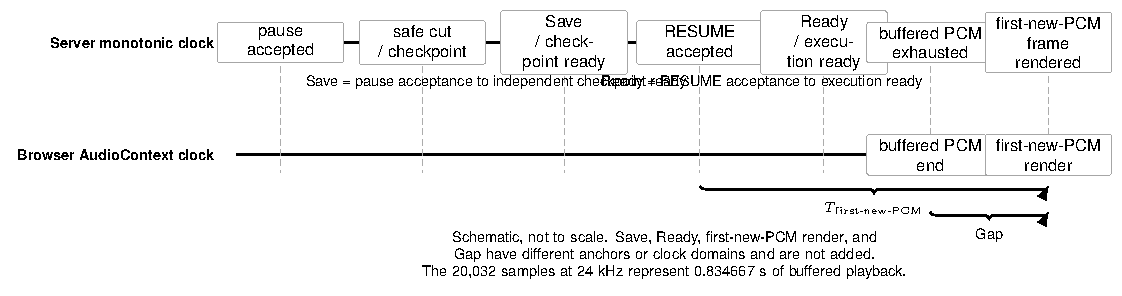
\includegraphics[width=\linewidth]{figures/fig_timeline.pdf}
    \caption{联合挂起／恢复协议及测量端点。图示不按时间比例绘制，分别显示服务端和浏览器时钟线：
    Save和Ready属于服务端区间，首个新PCM渲染和Gap使用浏览器AudioContext；这些区间具有不同锚点，不能相加。}
    \label{fig:timeline}
\end{figure}

\subsection{有界传输与完整性校验}
\label{sec:design_transfer}

状态适配器独立指定字节范围，M4使用pinned主机暂存、设备工作区和完成事件执行有界
 gather--transfer--scatter \citep{pytorchtransfer}；传输和SHA-256校验完成前，缓冲区不能复用，恢复后的KV还需在新映射中检查。
这些检查确认字节完整性，式~\eqref{eq:publish_guard}决定能否发布；payload、pinned暂存、进程RSS和GPU分配
属于不同统计口径。优化与同步路径保持相同检查点内容、恢复义务、模型计算和采样语义，打包只改变
搬运成本。共享权重、执行arena和传输工作区单独计量，部分卸载与联合卸载采用同一续算合同。

\section{实验}
\label{sec:experiments}

\subsection{实验环境}
\label{sec:exp_setup}

为全面评估所提出的全双工服务运行时在功能正确性、恢复效率和
交互服务能力方面的表现，本文在固定的硬件和执行配置下开展实验。
所有实验均使用两张A100-SXM4-40GB GPU，其中模型执行和声学执行
分别部署，共享模型权重保持常驻。实验主要从三个方面展开分析：
冷恢复，考察释放请求私有状态后的恢复连续性及时延--资源权衡；
传输与校验，隔离固定恢复合同下的检查点传输与校验开销；交互与外部协议，考察不同全双工
事件下的交互表现以及不同协议所带来的端点差异。各实验的具体
数据组织、对比策略、评价指标和统计分母将在对应小节中分别说明。

\subsection{冷恢复：正确性及时延--资源权衡}
\label{sec:cold_resumption}

冷恢复实验在两张A100-SXM4-40GB GPU上完成，负载采用冻结的公开
HumDial-FDBench测试归档中的语句级样本\citep{humdial2026,humdialdataset2026}。
该实验共统计96条运行记录。我们比较Hot、
Rebuild、Joint和Hybrid四种状态恢复策略，并重点考察恢复连续性、
首个新计算PCM渲染区间、post-buffer Gap以及状态恢复所产生的资源开销。
各策略的详细运行端点统计及其来源见附录。

测量端点使用两条独立时钟线。Save、RESUME接受和Ready使用服务端单调
时钟；Worklet恢复、缓存PCM耗尽和首个新计算PCM渲染使用浏览器
AudioContext时钟。主指标定义为
\begin{equation}
 T_{\mathrm{first\text{-}new\text{-}PCM}}
 = t_{\mathrm{new}}
   - t_{\mathrm{W,resume}} .
 \label{eq:first_new_pcm}
\end{equation}
Save是从暂停接受到独立检查点就绪的区间，Ready是从RESUME接受到执行就绪的区间，
Gap是从缓存PCM耗尽到首个新计算PCM的区间。
这些区间具有不同锚点，不能相加构成端到端时延；12.5秒来自逐运行配对的
主指标差值，而不是描述性表格中位数之差。

\begin{table}[H]
\centering
\caption{冷恢复的主要连续性、时延和资源结果。表中保留技术连续性结果、
首个新PCM渲染端点、相对Rebuild的配对减少量以及独立的E2资源口径；数值单位为秒或MiB。
valid/scheduled保留全部计划运行；详细Save、Ready、Gap、失败标签和来源记录见附录。}
\label{tab:cold_main}
\scriptsize
\setlength{\tabcolsep}{2.8pt}
\begin{tabular*}{\columnwidth}{@{\extracolsep{\fill}}lcccc@{}}
\toprule
指标 & Hot & Rebuild & Joint & Hybrid \\
\midrule
状态/恢复边界
& \shortstack[l]{保留活动上下文；\\时延参考}
& \shortstack[l]{释放私有状态；\\顺序重建}
& \shortstack[l]{释放私有状态；\\联合检查点}
& \shortstack[l]{释放模型/KV；\\保留声学状态} \\

连续性通过；有效/计划
& \shortstack[l]{24/24；\\24/24}
& \shortstack[l]{23/24；\\23/24}
& \shortstack[l]{24/24；\\24/24}
& \shortstack[l]{21/24；\\21/24} \\

E1首个新PCM渲染 (s)
& 1.184
& 14.451
& 1.899
& 1.349 \\

E2首个新PCM渲染 (s)
& 1.168
& 14.400
& 1.872
& 1.315 \\

相对Rebuild的配对减少量 (s)
& \textit{N/A}
& 0.000
& \shortstack[l]{E1: 12.547（10/11）\\E2: 12.507（13/13；12组）}
& \shortstack[l]{E1: 12.517（8/11）\\E2: 13.000（13/13；12组）} \\

E2检查点载荷 (MiB)
& \textit{N/A}
& \textit{NM}
& 672.207
& 22.416 \\

E2受管理pinned缓冲 (MiB)
& \textit{N/A}
& \textit{NM}
& 256
& 128 \\

E2 CPU持有RSS (MiB)
& 10534.685
& 10551.084
& 11477.773
& 10699.230 \\

E2声学GPU净回收 (MiB)
& 0.000
& 649.702
& 585.702
& 0.000 \\

E2模型GPU净分配变化 (MiB)
& 0.000
& -3.511
& +60.489
& +60.489 \\
\midrule
\multicolumn{5}{l}{
\scriptsize 计划运行：96条；技术通过：92条；每策略分母：E1 11 + E2 13 = 24
} \\
\bottomrule
\end{tabular*}

\vspace{1mm}
\begin{flushleft}
\scriptsize
注：连续性通过要求当前request/generation/permit有效，模型、bridge、
声学状态及progress/RNG校验通过，post-cut token/PCM后缀完整，输入/取消/
交付账本单调，无过期或重复输出，并且未来输入/control和数值设置匹配。
四种策略共享模型、切面、resume信号、播放器和连续性合同；Hybrid只改变
驻留边界，因此与Joint的比较是匹配条件下的时延--资源权衡。配对单元格
报告首个新PCM渲染的正向减少量；E2包含13个计划配对中的12个来源组，
E1报告可评价配对数。\textit{N/A}表示该策略不触发相应事件，
\textit{NM}表示冻结清单中没有对应测量；二者都不表示零。不同资源口径
彼此独立，不能直接相加。端点定义和Gap统计见附录。
\end{flushleft}
\end{table}
\FloatBarrier

表~\ref{tab:cold_main}汇总了四种状态恢复策略的连续性、主要时延
和资源开销。矩阵包含96条计划运行和92条技术通过记录；每个策略的
分母为24条（E1为11条，E2为13条）。表中的通过是技术连续性合同，
不等同于语义回答质量。Joint恢复的状态包括模型KV/non-KV状态、
待处理bridge内容、StreamingDecoder和Token2Wav连续状态、Flow / HiFT
缓存、实际随机上下文、stage progress以及请求身份和绑定描述符。
已接受输入、取消和交付事实保存在独立的单调账本中，不被旧检查点覆盖。

Hot保留活动上下文，因此只是时延参考，不满足冷释放。Rebuild释放
请求私有状态，并执行本文作为严格参考的顺序完整历史重建。Hybrid
释放模型/KV状态，但保留必要声学状态，是部分释放策略，而不是第二个
Joint实现。四种策略仍共享同一模型、切面、输入、resume信号、未来
input/control、播放器、校验合同和计划矩阵，因此Joint与Hybrid的比较
是在匹配条件下比较明确驻留边界带来的时延--资源权衡。

配对减少量来自匹配记录。Joint在E1的11个计划配对中有10个可评价，
首个新PCM渲染区间减少12.547\,s；E2为13/13个可评价配对、12个来源组，
减少12.507\,s。Hybrid对应为E1的8/11个配对、减少12.517\,s，以及
E2的13/13个可评价配对、12个来源组，减少13.000\,s。这些数值不是两个未配对总体中位数
相减得到的；附录报告对应的Gap中位数，并采用同generation缓存耗尽后的定义。

资源数据说明了这一权衡的成本和统计口径。E2中Joint和Hybrid的独立
检查点载荷为672.207和22.416\,MiB，受管理pinned缓冲为256和128\,MiB，
CPU持有RSS为11477.773和10699.230\,MiB。Rebuild在冻结清单中没有
对应检查点载荷事件，因此标记为NM而不是零；Hot保留活动状态，因此标记
为N/A。模型GPU净分配变化为正表示净增加，为负表示净回收；各资源口径
彼此独立，不能直接相加。

\subsection{吞吐量与扩展性}
\label{sec:throughput}

\begin{figure*}[t]
  \centering
  \includegraphics[width=0.32\linewidth]{fig3a.pdf}\hfill
  \includegraphics[width=0.32\linewidth]{fig3b.pdf}\hfill
  \includegraphics[width=0.32\linewidth]{fig3c.pdf}
  \caption{\textbf{校准后的端到端吞吐量随负载变化。}
  (a) 原生 Lychee-FD 与 DuplexPilot 的成对场景；候选/基线比值锚定于已测 APR/Affinity 运行。
  (b) 同一成对场景中首个输出 P90 随到达负载的变化；曲线为 5 次重复运行的均值，阴影表示四分位距。
  (c) Lychee-FD 服务栈上随最大模型 batch $B_{\max}$ 变化的吞吐扩展性。}
  \label{fig:throughput}
\end{figure*}

我们首先分析基于实测比值校准的 DuplexPilot 负载相关吞吐场景，该场景运行在原始 Lychee-FD 服务栈上。图~\ref{fig:throughput}(a) 显示，在 3--7 sessions/min 的低负载区间，吞吐量主要跟随到达率，候选由于启动路径略低于原生系统。进入容量受限区间后，两条曲线开始分离：在 13 sessions/min 时，校准场景中 DuplexPilot 为 11.38 sessions/min，Lychee-FD 为 10.88；在 15 sessions/min 时为 11.93 对 11.34；在 18 sessions/min 时为 12.25 对 11.62。在最高负载点，测得的 C/N16 锚点反转了排序：DuplexPilot 为 11.26，而 Lychee-FD 为 11.83。因而，成对比值同时包含增益和回退，不能概括为普遍吞吐优势。

图~\ref{fig:throughput}(b) 展示了这些吞吐量背后的时延权衡。在最低负载点，DuplexPilot 的首个输出 P90 较高（6.63 s 对 4.14 s）；在中负载区间时延略低（13 sessions/min 时为 8.23 s 对 8.44 s），而在最高负载点 P90 又更高（24 sessions/min 时为 18.77 s 对 17.80 s）。四分位阴影展示了重复运行之间的波动，同时避免把单次合成运行误当成独立工作点。这样可以把吞吐量变化与端点响应速度结合起来解释。

最后，图~\ref{fig:throughput}(c) 展示了同一服务栈中模型 batch 上限的影响。相对于各自的 $B_{\max}=1$，DuplexPilot 在 $B_{\max}=2$ 时达到约 1.20，并在约 1.21 附近饱和；Lychee-FD 达到约 1.18。两者差距较小且较早饱和，与已测成对比值一致：提高上限能够恢复部分混批机会，但不能保证端到端吞吐单调增加。

\subsection{传输与校验效率}
\label{sec:transfer}

为进一步分析检查点传输路径的效率，我们在相同的负载实例和恢复合同
下比较Sync与Optimized两种实现。两种实现使用相同的状态载荷、输入
来源、重复过程、接收端校验和接受规则。Sync表示同步完成检查点传输
和接收确认的路径，Optimized表示采用打包传输、传输与校验重叠的
优化路径。因此，该实验只改变检查点传输与校验的实现方式，不改变
恢复语义和后续执行过程。我们主要统计状态从发送端开始传输到接收
端达到就绪状态之间的时间，并同时记录暂停RSS和采样峰值RSS的变化。

在所有归档的匹配运行实例中，Optimized的传输至就绪时间均早于Sync。
Optimized相对于Sync的绝对减少量中位数为0.533\,s，逐实例相对减少量
的中位数为16.00\%。其中，逐实例相对减少量定义为
\[
    r_i =
    \frac{T_i^{\mathrm{Sync}}-T_i^{\mathrm{Optimized}}}
      {T_i^{\mathrm{Sync}}},
    \qquad
    T_i=t_{i,\mathrm{receiver\ ready}}-t_{i,\mathrm{state\ transmission\ start}}.
\]
采用逐实例相对减少量而不是两个配置整体中位数之比，可以避免不同
负载实例之间的时延差异改变总体结果的解释。所有匹配实例均获得
正向收益，说明该优化并非只在少数特殊负载上有效，而是能够稳定地
减少检查点传输路径中的等待时间。

传输效率的提升伴随着额外的内存开销。与Sync相比，Optimized的暂停
RSS和采样峰值RSS配对增加中位数分别为243.2和182.2\,MiB。这一
开销主要来自状态打包、暂存和接收端校验过程中需要保留的中间数据。
因此，Optimized体现的是传输等待时间与CPU内存占用之间的工程折中：
在恢复合同保持不变的情况下，打包和重叠校验能够缩短检查点传输时间，
但需要额外的主机内存支持。16.00\%是逐实例相对减少量的中位数，
不能解释为配置中位数之比，也不能作为额外倍率直接叠加到冷恢复
实验中的时延减少量上。该批次没有测量Worklet恢复、首个新PCM渲染、
播放结束或端到端恢复时延。

\subsection{交互与外部协议}
\label{sec:interaction}

为考察运行时在全双工交互场景中的状态转移和输出行为，我们采用
公开HumDial-FDBench测试归档整理的受控交互负载，并使用FD-Bench风格的事件定义
\citep{humdialdataset2026,fdbench2025}，覆盖普通回复、
用户插话、反向通道和停顿等事件类型。内部路径使用固定的事件定义、
输入节奏和统计分母，并按照SRR、SIR、SRIR、EIR、FSED和IRD等指标
进行评估。与此同时，我们记录vLLM-Omni原生热重附着和LiveServe
风格预加载路径的端点行为，用于分析不同协议下ready、ACK和首个
PCM输出之间的关系。外部路径的模型、输入调度和计时端点与内部
受控实验不同，因此只作为协议参照，不作为匹配基线。

本先导中，SRR定义为符合条件的非打断问句中成功回复的数量除以
符合条件的非打断问句总数；SIR为实际打断机会中检测到正向打断的
数量除以实际打断机会总数；SRIR为实际打断机会中成功完成打断响应
的数量除以实际打断机会总数；EIR为有效事件窗口中助手过早进入的
数量除以有效事件窗口总数。FSED是用户语音结束到匹配回复开始播放
的带符号时延，IRD是用户插话开始到助手上一段语音结束的带符号时延。
因此下文每个比例都显式给出分子和分母。每条路径的六个source group
作为source-level bootstrap重采样单位，共进行200,000次百分位数
bootstrap；时延只使用有效事件观测，不对缺失值插补。

表~\ref{tab:interaction_protocol}汇总了内部受控路径和外部协议
参照的关键测量口径。最终manifest包含6个已完成source group、10个
有效问句、3个实际打断机会，且没有无效或取消的运行。受控路径的
SRR为$7/7=100.0\%$（95\% bootstrap CI为$100.0$--$100.0$），
SIR为$3/3=100.0\%$（[100.0,100.0]），SRIR为$3/3=100.0\%$
（[100.0,100.0]），EIR为$4/10=40.0\%$（[25.0,50.0]），FSED中位数
为4445.9\,ms（$n=10$，[3714.6,5582.8]），IRD中位数为278.2\,ms
（$n=3$，[266.6,898.9]）。没有无效／取消运行或不可评价source group；
无效／取消事件行同样为0，评分器排除了2条非指标反向通道记录，
reply timeout为0。逐source重复
结果见表~\ref{tab:interaction_repeats}及机器可读文件
\texttt{data/final/interaction\_metrics\_per\_repeat.csv}，bootstrap细节见
\texttt{data/final/interaction\_metrics\_bootstrap.csv}。原生Omni参照的
SRR为$6/7=85.7\%$（bootstrap CI为$[66.7,100.0]\%$），SIR为$3/3$，
SRIR为$3/3$，EIR为$9/10=90.0\%$（$[70.0,100.0]\%$），FSED中位数
为635.5\,ms（$n=9$，[58.5,1324.7]），IRD中位数为2068.3\,ms
（$n=3$，[564.1,3444.6]）。这是现有的原生交互参照，不是naive-cold
或同模型匹配基线。对于vLLM-Omni原生
热重附着，记录中的请求至ACK时间为1.512和1.421\,ms，首PCM接收
时间为725.412和776.220\,ms；PCM序号没有出现缺失或重复，但现有
记录无法确定首个返回PCM所处的具体产生阶段。LiveServe式组件提前
约9.9\,s准备20和15\,MiB的KV状态，使ready时间分别提前约56.65
和100.01\,ms；然而以共同源窗口为计时锚点时，首个新PCM的接收
时间分别晚23.7和36.4\,ms。

相对于原生Omni交互参照，Lychee/DuplexPilot减去Omni的原始描述性
差异为：SRR增加14.3个百分点，SIR为0，SRIR为0，EIR减少50.0个
百分点，FSED增加3810.4\,ms，IRD减少1790.1\,ms。这些不是因果基线
估计，因为两条路径的模型、输入调度和计时端点不同；本批次没有
记录naive-cold交互基线。Lychee/DuplexPilot固定采用400\,ms块末端
输入交付；没有配对的200\,ms或零量化对照，因此无法估计400\,ms的
因果影响。该调度最多引入一个400\,ms的边界量化（若输入均匀到达，
期望约200\,ms），所以报告的FSED和IRD包含这一协议影响。

这些结果表明，ready时间提前并不必然意味着用户能够更早获得可听
输出。Lychee/DuplexPilot采用400\,ms块末端输入，而Omni客户端
采用200\,ms先发送再等待的输入协议；不同协议中的ready、ACK、首
PCM接收和PCM产生分别对应交互流水线中的不同阶段。因此，外部
协议观察只能用于说明端点关系和协议边界，不能与内部受控结果合并
为统一的冷恢复性能排名。

\begin{table*}[t]
\centering
\caption{受控交互路径和外部协议参照的测量口径与观察结果。外部
协议仅作为观察性参照，不作为匹配基线。}
\label{tab:interaction_protocol}
\scriptsize
\setlength{\tabcolsep}{4pt}
\begin{tabular}{p{0.18\textwidth}
                p{0.22\textwidth}
                p{0.27\textwidth}
                p{0.25\textwidth}}
\toprule
路径或协议
& 数据与输入方式
& 主要端点或指标
& 观察结果与可比性说明 \\
\midrule

Lychee/DuplexPilot
受控路径
&
HumDial-FDBench公开测试音频与FD-Bench风格事件定义；
普通回复、用户插话、反向通道和停顿；
400\,ms块末端输入
&
SRR、SIR、SRIR、EIR、FSED和IRD；
SRR $7/7$、SIR $3/3$、SRIR $3/3$、
EIR $4/10$；FSED 4445.9\,ms（$n=10$）、
IRD 278.2\,ms（$n=3$）。bootstrap 95\% CI：
EIR [25.0,50.0]\%，FSED [3714.6,5582.8]\,ms，
IRD [266.6,898.9]\,ms。6次重复；
无效／取消 $0/6$，reply timeout为0
&
内部受控结果。事件定义、输入节奏和
统计分母固定；统计10个有效问句和3个
打断机会。固定400\,ms交付调度已包含在
时延数值中，没有配对200\,ms消融 \\

vLLM-Omni
原生热重附着
&
200\,ms先发送再等待；
原生Omni输入协议
&
请求至ACK：
1.512 / 1.421\,ms；

首PCM接收：
725.412 / 776.220\,ms
&
PCM序号没有缺失或重复；
首个返回PCM的具体产生阶段未知。
模型、输入调度和端点定义不同，
不作为匹配基线 \\

LiveServe-style
预加载路径
&
提前准备KV状态；
20 / 15\,MiB；
约9.9\,s提前执行
&
ready时间提前：
56.65 / 100.01\,ms；

共同源窗口锚点下首个新PCM接收：
晚23.7 / 36.4\,ms
&
更早ready不等于更早可听输出。
该路径与内部实验的模型、调度和端点
定义不同，只用于说明协议层次之间的
时间关系 \\
\bottomrule
\end{tabular}
\end{table*}

\section{讨论与总结}
\label{sec:discussion_conclusion}

\subsection{局限性分析}
\label{sec:limitations}

本文方案的首要适用前提是音频生成侧能够提供可拆分、可导出和可
恢复的内部状态。只有当声学后端能够显式暴露必要的缓存、执行进度、
待处理输出以及相关运行时上下文时，DuplexPilot才能完成状态保存、
传输、重新绑定和继续执行。如果音频生成过程被封装为无法中断、
无法导出和无法恢复的黑盒操作，则该方案无法直接适用。因此，
DuplexPilot并不是面向任意音频生成后端的通用外挂优化，其有效性
依赖于声学状态的可观测性和可恢复性。

本文将DuplexPilot迁移到vLLM-Omni后的测量结果，也不能代表
vLLM-Omni原生系统能够达到的最优性能。相关结果受到当前迁移实现、
输入节奏、调度配置、模型执行路径以及端点定义的共同影响。由于
不同系统在模型实现、KV管理、声学执行方式和输出协议方面存在差异，
本文中的vLLM-Omni结果只能作为协议和端点层面的观察，不能作为对
vLLM-Omni整体性能上限的判断，也不能与内部受控结果直接构成统一
的系统排名。

此外，当前实验主要覆盖正常的状态保存、传输、恢复和继续执行过程，
对故障场景的覆盖仍不充分。检查点传输中断、部分恢复、设备或worker
失效、checkpoint损坏、状态版本不兼容以及恢复过程中的回滚和原子
提交等问题，尚未得到系统验证。因此，当前结果主要说明运行时在
正常恢复路径下的状态管理能力，面向长期运行服务的故障隔离、失败
恢复和状态格式演化机制仍需要进一步研究。

\subsection{总结}
\label{sec:conclusion}

本文的核心工作是将全双工服务中的音频生成状态从隐含的执行上下文
转化为运行时可以显式管理的对象。在音频生成状态能够被拆分和恢复
的前提下，运行时可以对逻辑请求状态、模型执行状态、桥接状态和
声学执行状态进行独立管理，从而支持请求私有资源释放后的状态恢复
和全双工连续执行。该方法的价值不在于为某个特定系统提供一个固定
的性能倍率，而在于建立了一种面向全双工服务的状态虚拟化抽象。
后续工作将重点围绕更通用的声学状态接口、面向故障的恢复机制以及
统一公平的跨系统评测协议展开。

\section*{AI 使用声明}
AI协助数据分析、图表生成和英文表述修订。

\section*{可复现性声明}
公开源码仓库位于
\url{https://github.com/ICALab-nsccjn/DuplexPilot}。仓库包含核心运行时
与检查点合同、公开测试、工作负载生成器、分析工具、配置说明，以及
用于构建本文的 LaTeX 源码。生成日志、中间实验结果、归档记录和模型
检查点有意不上传。公开数据集以其上游地址、版本和校验和记录；超过
GitHub 普通文件大小限制的数据文件不直接纳入仓库。若第三方检查点因
许可不能重新分发，仓库会提供其公开下载地址、精确版本、许可信息和
校验和。发布的脚本和论文图表因此暴露可复现的实现接口，但不声称公
开私有运行轨迹或受限权重。

\bibliographystyle{plainnat}
\bibliography{references}

\clearpage
\appendix
% 放在参考文献之后。
% 所需宏包：booktabs、array。
% 整体替换旧版附录，不要追加到旧版后面。
% 每个语言版本的主稿只使用一次 \appendix。

\clearpage
\appendix

% 附录A
\section{复现与测量}
\label{app:protocol}

\paragraph{复现材料。} 可复现性声明所述 GitHub 发布包将提供可执行源码、
配置与依赖清单、运行命令、图表生成脚本和机器可读结果表，以便重新生成
论文中的结果。缺失或不可评价字段将明确报告，不以插值替代。

\paragraph{数据来源与命名。} 本文使用公开的
\emph{HumDial-FDBench}测试归档；正式论文为Wang等人
\citep{humdial2026}，数据页单独引用为\citep{humdialdataset2026}。
官方划分为Train 8,898、Dev 1,800和Test 5,000条，覆盖九类场景；公开测试归档
另含4,100个用于评分的clean文件。本文冻结的Hugging Face revision为
\texttt{ed1770a6265ffe9f0e5cd999290936ccab43482b}，数据卡标注Apache-2.0。
冻结归档中的WAV为单声道、16-bit PCM、16\,kHz；本文直接使用发布的WAV字节和
JSON标注，不做项目内重采样、降噪、响度归一化或合成混音。样本ID保留归档路径
\texttt{test/\{en,cn\}\_test\_nondev/\{scenario\}/\{base\_id\}[\_add].wav}，
clean文件是独立的评分参照。运行时cut从选定完整WAV在实验固定的非空状态边界生成，
属于项目派生回放切面，不是官方HumDial-FDBench片段或榜单分数；cut ID、时间戳、
来源成员和哈希绑定在运行manifest中。该发布物是人工录制的表演语音，不是TTS；
公开论文和数据卡没有说明去标识化或说话人匿名化流程，因此本文不宣称音频已经去标识化。

全文统一使用：\emph{FD-Bench}（Peng等）是独立基准，不使用无连字符简称；
“HumDial-FDBench”仅作为HumDial官方数据集标识保留；
\emph{Full-Duplex-Bench}指Lin等人的家族，其中v1和v1.5是离线版本，
\emph{Full-Duplex-Bench-v2}是后续实时框架；\emph{HumDial-FDBench}是基于v1.5协议
构建的HumDial基准，既不是FD-Bench数据集，也不是Full-Duplex-Bench-v2。
本文改编的事件定义统一称为“FD-Bench风格”。


冷恢复实验使用相同的Lychee-FD模型与本地Token2Wav后端
\citep{lychee2026}，
在两张A100-SXM4-40GB GPU上分别部署模型执行和一个声学lane。
共享权重保持常驻，
每组比较内部匹配模型、采样、数值、输入和播放配置。
复现需要实际执行的源码、依赖与配置清单，包括归档补丁，
不能仅依据仓库commit。

最终矩阵包含12个来源组、四种策略和两次重复，共96次执行。
E1包含44次，E2包含52次，两个环境分别统计。
测量批次包含24个待处理语音token，以及20,032个24\,kHz缓存PCM样本。
这些数值描述预定义非空切面，而非自然会话状态分布。
名义挂起时间为30秒，但时延采用实际事件计量。
新音频渲染从Worklet恢复开始，
计量至同一AudioContext中首个新计算PCM帧被渲染，
缓存音频续播不属于新计算。主指标为
\[
T_{\mathrm{first\text{-}new\text{-}PCM}}
=t_{\mathrm{new}}-t_{\mathrm{W,resume}}。
\]
Save使用安全暂停到资源就绪的区间，Ready使用RESUME接受到执行发布的区间，
二者均采用服务端单调时钟；Gap使用浏览器时钟定义为
$\max(0,t_{\mathrm{new}}-t_{\mathrm{buffered\text{-}end}})$。
这些端点不是串行片段，不能相加。

配置统计先在同来源、同环境内汇总具有对应端点的重复，
再取来源间中位数。配对差先匹配来源、重复和环境；缺失值不以零替代。
冷恢复、传输、吞吐量和交互批次分别保留身份，不合并统计。

最终矩阵包含96条计划运行，其中92条通过技术合同。Rebuild保留1条
E1暂停后原生浏览器帧重叠取消；Hybrid保留3条E1失败（两条帧重叠
取消和一条冻结切面/首个PCM观测轮次不匹配）。Hot和Joint没有失败，
E2全部通过技术合同。Hot和Rebuild没有对应的检查点、pinned缓冲或
GPU工作区测量事件，主表分别标记为N/A或NM，不填零。system pinned、
$L_{\mathrm{useful}}$和$J(T)$不属于本轮冷恢复合同，明确标记为未评价。


% 附录B
\section{联合状态与恢复验证}
\label{app:state_contract}

表\ref{tab:app_state_contract}总结联合恢复边界。
计算状态可以恢复，而已接受输入、取消决定与交付记录保持当前值。
这一区分在请求粒度上应用一致快照与回滚恢复原则
\citep{chandy1985,elnozahy2002}。

\begin{table}[tbp]
    \centering
    \small
    \setlength{\tabcolsep}{5pt}
    \caption{
        状态覆盖与恢复义务。
        外部记录持续保留，不被旧检查点副本覆盖。
    }
    \label{tab:app_state_contract}
    \begin{tabular}{
        @{}
        >{\raggedright\arraybackslash}p{0.20\linewidth}
        >{\raggedright\arraybackslash}p{0.73\linewidth}
        @{}
    }
        \toprule
        状态类别 & 内容与恢复义务 \\
        \midrule
        模型
        & 有效KV、非KV历史、处理器／控制状态、采样上下文和逻辑位置。
          将数值恢复至合法映射，并重建活动绑定。 \\
        桥接
        & 已产生但未消费的token、部分缓冲、
          初始化／flush状态和待提交输出。
          保留内容与消费顺序。 \\
        声学
        & StreamingDecoder与Token2Wav连续状态、
          Flow / HiFT缓存、实际随机上下文和待提交PCM。
          恢复兼容的执行上下文。 \\
        身份与进度
        & 请求、generation、状态版本、cut、lease epoch、sequence、
          producer epoch和各阶段水位。
          根据当前生命周期验证归属。 \\
        外部记录
        & 已接受输入、取消决定及交付／渲染区间。
          保留当前事实，拒绝过期提交。 \\
        \bottomrule
    \end{tabular}
\end{table}

捕获阶段先建立一致切面与独立主机检查点，
再交还请求私有资源。
恢复阶段准备合法映射、重建绑定并验证各参与阶段状态，
之后才允许执行和输出。
发布时重新检查当前generation、版本和取消状态；
失败或已取消的恢复不被发布。
恢复已保存的输入消费位置，不会覆盖检查点之后收到的输入。

请求身份回归区分物理输出顺序$[A,B]$
与仅包含$B$的采样选择。
request ID查找取得$B$对应的side output，
而不是物理第零行的输出。
独立归档检查还覆盖桥接待处理内容、发布前拒绝和请求局部取消。
完整token与波形比较以匹配的输入／控制历史及数值配置为条件，
不代表语义正确，也不保证任意kernel的无条件确定性。

\paragraph{协议证明义务。}
协议信封$q$包含五个字段：\textit{request\_id}、\textit{generation}、\textit{state\_version}、
\textit{cut\_id}和\textit{lease\_epoch}；每条记录再附带\textit{sequence}和
\textit{producer\_epoch}。证明采用如下归纳。初始状态只有一个归属者，
已产生集和已消费集均为空。SAVE在切面线性化点前关闭全部写入者，因此检查点内记录具有相同$q$；
排空在途提交后，检查点与队列恰好划分已产生未消费集合。RESUME只有在读取当前账本水位后才安装
新的lease epoch。之后每个提交只有在完整信封等于当前permit时接受，账本更新与队列位置推进原子完成。

因此，请求ID不匹配的记录会被拒绝，归属保持不变；token要么在检查点中，要么由消费者事务恰好移除一次，
桥接守恒保持；输入、取消和交付水位只增不减，账本单调性保持。generation、state version与lease epoch
共同拒绝迟到worker及ABA lease复用。消费者只接受下一个sequence，故PCM前缀／顺序由归纳得到。
PUBLISH是离开RESTORING的唯一转换，且只在这些检查完成后开放，因此无效状态不能执行或可见。
任一前提失败都转入\textsc{Aborted}，不会发布半恢复状态，也不会回滚外部事实。

两个线性化点在trace中可观测：\textsc{Cut}是原子关闭并快照的事件，\textsc{Restore}是原子安装新lease
和permit的事件。取消在线性化时写入账本；恢复若观察到该记录则中止，而更晚的取消会在下一次提交前使
permit失效。上述规则分别覆盖切面不一致、版本过期、ABA lease、迟到worker、桥接重复消费、PCM乱序、
取消／恢复竞争及检查点后的新输入，不依赖物理worker身份。

\begin{algorithm}[tbp]
\caption{逻辑请求$r$的保存／恢复协议。}
\label{alg:save_resume}
\begin{algorithmic}[1]
\Require 当前信封$q$、状态$(M,B,A)$和外部账本$L$
\Ensure 发布permit，或进入不可执行的中止状态
\State 原子关闭输入、token生产和输出发布入口
\State 递增\textit{state\_version}并分配\textit{cut\_id}
\State 在支持的边界暂停$M,B,A$并排空在途提交
\If{存在信封不同于$q$的记录}
    \State 拒绝该记录并中止捕获
\EndIf
\State 在\textsc{Cut}线性化点执行$K\gets\Call{Snapshot}{M,B,A,L,q}$
\If{$\neg\Call{CheckJoint}{K}$}
    \State 保留原资源；\Return \textsc{Aborted}
\EndIf
\State 释放私有资源并将$r$标为挂起
\State 读取当前$L$；若取消或低于输入／取消／交付水位则拒绝
\State 分配新的\textit{lease\_epoch}并合并切面后的输入
\State 从$K$重绑定$M,B,A$
\If{$\neg\Call{CheckJoint}{M,B,A,L,q}$}
    \State 丢弃未发布状态；\Return \textsc{Aborted}
\EndIf
\State 在\textsc{Restore}点原子安装新lease和permit
\While{$r$仍在执行}
    \If{提交信封不等于$q$，或PCM序列不是下一个前缀值}
        \State 丢弃该提交
    \Else
        \State 原子追加账本记录并推进消费位置
    \EndIf
\EndWhile
\State \Return \textsc{Published}
\end{algorithmic}
\end{algorithm}


% 附录C
\section{补充性能结果}
\label{app:performance}

表\ref{tab:app_latency}补充正文的测量端点。
表中同时报告保存、就绪、首个新PCM渲染和间隔，
每项均保留自己的起止锚点。
各指标保留自己的起止端点，
不与其他区间相加构造新的端到端指标。

\begin{table}[tbp]
    \centering
    \small
    \setlength{\tabcolsep}{6pt}
    \caption{
        补充冷恢复测量，单位秒。
        数值为对应环境内端点的来源级中位数。N/A表示事件不适用，NM表示
        没有对应测量；二者都不是零。第一组给出最新报告中完整96次运行
        分母下的策略级有效率；失败运行仍保留在分母中。
    }
    \label{tab:app_latency}
    \begin{tabular}{@{}llcrrrr@{}}
        \toprule
        环境 & 策略 & 有效/总数 & 保存 & 就绪 & 首个新PCM渲染 & 间隔 \\
        \midrule
        \multicolumn{7}{@{}l}{\emph{所有环境（最新96次运行批次）}} \\
        All & Hot     & 96/96 & \na & \na & \na & \na \\
        All & Rebuild & 92/96 & \na & \na & \na & \na \\
        All & Joint   & 96/96 & \na & \na & \na & \na \\
        All & Hybrid  & 96/96 & \na & \na & \na & \na \\
        \midrule
        E1 & Hot     & 11/11 & 0.004 & 0.001  & 1.184 & 0.349 \\
        E1 & Rebuild & 10/11 & 1.847 & 13.317 & 14.451 & 13.616 \\
        E1 & Joint   & 11/11 & 1.387 & 0.699  & 1.899 & 1.064 \\
        E1 & Hybrid  & 8/11  & 0.655 & 0.130  & 1.349 & 0.515 \\
        \midrule
        E2 & Hot     & 13/13 & 0.004 & 0.001  & 1.168 & 0.333 \\
        E2 & Rebuild & 13/13 & 1.926 & 13.250 & 14.400 & 13.565 \\
        E2 & Joint   & 13/13 & 1.387 & 0.700  & 1.872 & 1.037 \\
        E2 & Hybrid  & 13/13 & 0.696 & 0.136  & 1.315 & 0.480 \\
        \bottomrule
    \end{tabular}
\end{table}

最终批次的首个新PCM渲染区间比缓存后供给间隔多
$20{,}032/24{,}000=0.834667$秒。这是预定义缓存播放时长，
不是额外的时延项；二者是同一交付时间线的不同视角，不是独立改善。
E2中，Joint与Hybrid的独立检查点载荷分别为
672.207和22.416\,MiB，
受管理pinned缓冲分别为256和128\,MiB。
两者均保留模型设备工作区，使模型GPU净分配增加60.489\,MiB。
检查点大小、pinned存储、进程RSS和设备分配属于不同测量，
不能直接相加。

独立传输实验包含六个来源组、12对Sync/Optimized运行。
每对的相对降幅为
$(T_i^{\mathrm{sync}}-T_i^{\mathrm{opt}})/T_i^{\mathrm{sync}}$。
其中传输到接收端就绪区间的相对降幅中位数为16.00\%，绝对减少量中位数为0.533秒，
12对均为优化路径更快。该批次没有测量Worklet恢复、首个新PCM渲染、播放结束或端到端恢复时延。
额外暂停RSS与采样峰值RSS的配对增加中位数
分别为243.2和182.2\,MiB。
历史吞吐矩阵则对各负载／并发单元的逐次配对比值取均值。
其全部配置和重复应完整保留；
新吞吐测量作为独立批次处理。


% 附录D
\section{交互与外部协议}
\label{app:interaction}

自然交互先导采用FD-Bench风格的适配定义\citep{fdbench2025}。
SRR、SIR与SRIR的分母分别保留符合条件的非打断问句、
实际打断机会和成功打断事件。
EIR记录助手过早进入用户话轮。
FSED从用户语音结束计量至匹配回复开始播放，
IRD从用户插话开始计量至助手上一段语音结束。
时延保留正负符号。
显式CPU挂起不计作语音打断，
拼接PCM也不能替代真实渲染时间线。

导出的事件列按如下方式计算
$\mathrm{SRR}=k_{\mathrm{SR}}/n_{\mathrm{SR}}$、
$\mathrm{SIR}=k_{\mathrm{SI}}/n_{\mathrm{SI}}$、
$\mathrm{SRIR}=k_{\mathrm{SRI}}/n_{\mathrm{SRI}}$和
$\mathrm{EIR}=k_{\mathrm{EI}}/n_{\mathrm{EI}}$；某指标列缺失时，该事件
不进入该指标分母。每条受控路径有10个有效问句、3个实际打断机会，
6次重复中无效／取消运行数为0。唯一非零的失败相关字段是Omni的
1次reply timeout，该记录不产生FSED观测，因此该路径FSED有效$n=9$。
正文区间是source-level bootstrap区间（对6个source group重采样
200,000次，seed为20260926）；有效bootstrap次数保留在
\texttt{interaction\_metrics\_bootstrap.csv}中。

共享Lychee/DuplexPilot在线路径属于同一实现，
不是两个独立基线。
该路径采用400\,ms块末端输入，
Omni客户端采用200\,ms先发送、再等待的输入方式；
模型和实际打断暴露状态也不同。
因此，先导描述应用行为，不用于隔离冷恢复影响。
此前听音反馈只适用于已经审阅的案例，
不扩展到未审阅先导输出。

两例vLLM-Omni原生热重附着\citep{omnidoc}
的请求至ACK分别为1.512和1.421\,ms，
首PCM接收分别为725.412和776.220\,ms。
两例记录中的PCM序号没有缺失或重复，
但首个返回PCM的产生阶段未知。
LiveServe风格预加载组件\citep{liveserve2026}
提前约9.9秒准备20和15\,MiB KV。
其就绪分别提前约56.65和100.01\,ms，
但从共同源窗口计量的首新PCM接收分别晚23.7和36.4\,ms。
这些观察保留各自原生协议，
不构成统一的外部冷恢复比较。

\begin{table*}[t]
\centering
\scriptsize
\setlength{\tabcolsep}{3pt}
\caption{受控Lychee/DuplexPilot路径和原生Omni参照路径的逐source重复结果。比例为分子/分母；FSED和IRD为带符号播放层中位数（ms），括号内为有效$n$。每次重复均未出现无效或取消运行；反向通道排除是有意的非指标事件，不是失败。}
\label{tab:interaction_repeats}
\begin{tabular}{llccccrrcc}
\toprule
配置 & source group & SRR & SIR & SRIR & EIR & FSED (ms) & IRD (ms) & timeout & 无效/取消 \\
\midrule
Lychee & 0001\_0001 & 1/1 & -- & -- & 0/1 & 3666.4 (1) & -- & 0 & 0 \\
Lychee & 0001\_0003 & 1/1 & -- & -- & 0/1 & 3762.9 (1) & -- & 0 & 0 \\
Lychee & 0001\_0015 & 1/1 & 1/1 & 1/1 & 1/2 & 5582.8 (2) & 266.6 (1) & 0 & 0 \\
Lychee & 0001\_0025 & 1/1 & 1/1 & 1/1 & 1/2 & 5575.1 (2) & 278.2 (1) & 0 & 0 \\
Lychee & 0001\_0029 & 2/2 & -- & -- & 1/2 & 5808.0 (2) & -- & 0 & 0 \\
Lychee & 0001\_0031 & 1/1 & 1/1 & 1/1 & 1/2 & 3615.5 (2) & 898.9 (1) & 0 & 0 \\
\midrule
Omni & 0001\_0001 & 1/1 & -- & -- & 1/1 & -185.9 (1) & -- & 0 & 0 \\
Omni & 0001\_0003 & 1/1 & -- & -- & 1/1 & 1324.7 (1) & -- & 0 & 0 \\
Omni & 0001\_0015 & 1/2 & -- & -- & 2/2 & 302.9 (1) & -- & 1 & 0 \\
Omni & 0001\_0025 & 1/1 & 1/1 & 1/1 & 1/2 & 1507.4 (2) & 3444.6 (1) & 0 & 0 \\
Omni & 0001\_0029 & 1/1 & 1/1 & 1/1 & 2/2 & 1351.6 (2) & 564.1 (1) & 0 & 0 \\
Omni & 0001\_0031 & 1/1 & 1/1 & 1/1 & 2/2 & 1544.5 (2) & 2068.3 (1) & 0 & 0 \\
\bottomrule
\end{tabular}
\end{table*}


\end{document}





















